\section{Method}
\label{sec:method}

\subsection{Preliminaries: Projection Injection}\label{sec:method3.1}
%
\YW{
Unlike attention-based 3D generators such as TRELLIS~\cite{Xiang_2025_CVPR_Trellis}, which implicitly learn associations between image tokens and 3D queries, Pixal3D~\cite{li2026pixal3d} explicitly establishes 2D-3D spatial correspondence through back-projection, enabling high-fidelity image-to-3D generation.
%
% This approach enables high-fidelity image conditioning and provides explicit correspondences for transferring image features to 3D queries.
%
We adopt this projection-based conditioning principle, as its explicit spatial associations provide a suitable foundation for retrieving and adapting source appearance evidence across geometric changes.
% We adopt this projection-based conditioning principle, as its explicit spatial associations are suitable for identifying and adapting source appearance across geometric changes.
%
Given multi-view images $\{I_v\}_{v=1}^{V}$, the projected features at voxel $\mathbf{x}$ are aggregated as
%
\begin{equation}
    \mathbf{F}^{3D}(\mathbf{x}) =
    \frac{1}{V}\sum_{v=1}^{V}
    \operatorname{Sample}\left(
        \Phi(I_v), \pi_v(\mathbf{x})
    \right),
    \label{eq:projection_injection}
\end{equation}
%
where $\Phi$ denotes the image encoder, $\pi_v$ is the camera projection for view $v$, and $\operatorname{Sample}$ denotes bilinear sampling.
%
However, explicit geometric projection alone does not guarantee semantic consistency when the input views depict different shapes.
%
Consequently, features projected onto the same 3D query may originate from semantically unrelated object regions, leading to appearance misalignment.
%
We therefore preserve the target-view conditioning while adapting source appearance through semantic correspondence-guided feature aggregation and retargeting.
% However, explicit geometric projection alone does not guarantee semantic consistency when the input views depict different shapes.
% %
% As a result, visual features projected onto the same 3D query may originate from unrelated object regions, leading to appearance misalignment.
% % In our setting, the geometry-aligned target view and original source views represent different geometric states, such that direct feature aggregation may introduce appearance misalignment.
% %
% We therefore preserve the target-view conditioning while selectively adapting source appearance through semantic correspondence-guided feature aggregation and retargeting.
}






























\subsection{Data Construction: DeformNeXt-10k}\label{sec:method3.2}
%
\YW{
To supervise appearance retargeting across geometric variations, we construct \emph{DeformNeXt-10k} from textured 3D assets and hierarchical part annotations of PartNeXt~\cite{wang2026partnext}.
%
For each source object, we employ donor-guided GeoStyle~\cite{choi2026image} deformation with part-aware assembly constraints to generate diverse geometric variations.
%
The resulting candidates are screened for meaningful deformations and major geometric artifacts.
%
Importantly, each source mesh $M_0=(V_0,F,A_0)$ and its deformed counterpart $M_1=(V_1,F,A_0)$ share identical face connectivity and appearance attributes, including UV coordinates and materials.
%
This preserves exact surface correspondences through shared face indices and barycentric coordinates while retaining the original appearance.
%
We render both geometric states from calibrated viewpoints to obtain paired target and source observations for training.
%
The resulting dataset contains 10,165 paired deformations, providing correspondence supervision for semantic feature matching and supervised training of geometry-conditioned appearance retargeting.
}







































\subsection{VLM-Guided Target-View Editing}
\label{sec:method3.3}
%
\YW{
% Direct geometric manipulation can be difficult for diverse object deformations, while geometry-only controls may leave the visual condition inconsistent with the edited shape.
Direct mesh-based editing often requires explicit deformation constraints or optimization~\cite{yoo2024plausible,choi2026image}, while spatial geometry controls~\cite{fedele2026spacecontrol} may leave the original visual condition inconsistent with the edited shape.
%
These limitations make it challenging to achieve flexible geometric editing while maintaining geometry-image consistency.
%
To address this, we employ a vision-language model (VLM) to translate user-specified geometric modifications into a geometry-aligned target image.
%
Given an original target-view image $I_t^0$ and a desired geometric condition $\mathcal{G}^{\star}$, we obtain
%
\begin{equation}
    I_t^{\mathrm{edit}} =
    \mathcal{E}_{\mathrm{VLM}}
    \left(I_t^0,\mathcal{G}^{\star}\right),
    \label{eq:vlm_editing}
\end{equation}
%
where $\mathcal{E}_{\mathrm{VLM}}$ denotes the geometry-guided image editing process.
%
By leveraging the real-world commonsense knowledge of VLMs, this approach translates diverse geometry conditions into compatible edited target images.
% By leveraging the semantic and visual priors of VLMs, this approach expresses diverse geometric modifications as image-domain observations compatible with pretrained image-to-3D generation.
%
The edited target view serves as a structural anchor, while the original source views retain complementary appearance cues.
%
However, these observations have different geometry, requiring explicit appearance retargeting during 3D generation.
}








































\subsection{GEAR3D Framework}\label{sec:method3.4}

\YW{
Given the geometry-aligned target view and a set of original source views indexed by $\mathcal{S}$, \emph{GEAR3D} adapts source appearance evidence to the target geometric state within a pretrained projection-based 3D generator.
%
Let $V=|\mathcal{S}|+1$ denote the total number of conditioning views, including the target view.
%
Our framework consists of three components: semantic feature matching, matching-aware feature aggregation, and target-aware feature retargeting.
}

\begin{figure*}[t]
    \centering
    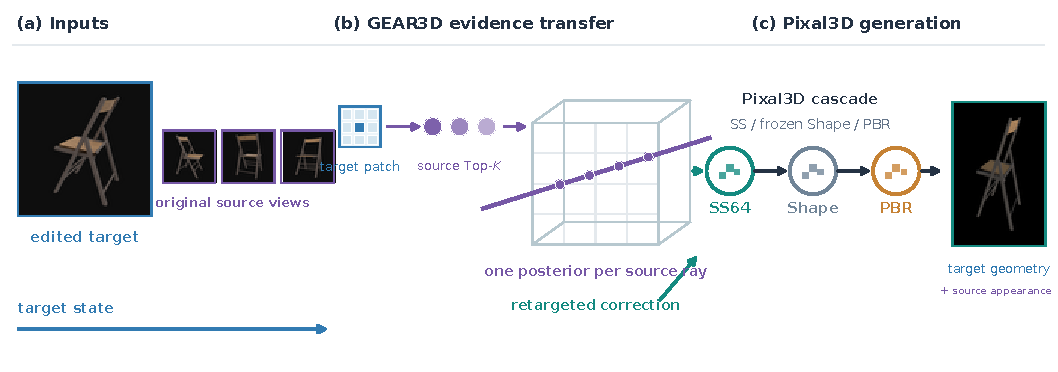
\includegraphics[width=\textwidth]{figures/paper-overall-v3.pdf}
    \caption{\textbf{GEAR3D overview.} An edited target view anchors the desired
    geometry, while three original views provide source appearance.  GEAR3D
    retrieves semantic source evidence, shares its posterior across the 3D
    sites on each source-camera ray, and injects only a residual source
    correction into the native SS64 conditioning carrier.  The result then
    follows the pretrained Pixal3D cascade with frozen Shape stages and a
    stage-specific PBR adapter.  Image panels are from an archived test case;
    correspondence glyphs are schematic.}
    \label{fig:gear3d-overview}
\end{figure*}



























\paragraph{Semantic Feature Matching.}
%
\YW{
To transfer source appearance across geometric variations,
we first establish semantic correspondences between the
geometry-aligned target view and the original source views.
%
We employ geometry-aware descriptors from a
frozen VGGT-$\Omega$~\cite{wang2026vggtomega} backbone
for correspondence estimation.
%
For each target patch, we retrieve the top-$K$ source
patch candidates based on feature similarity.
%
However, direct feature similarity may produce unreliable
correspondences under deformation and pose variations.
%
To improve matching accuracy, we adapt a lightweight
matching decoder~\cite{nordstrom2026romaomega} that contextualizes target descriptors
through cross-attention and refines candidate matching scores.
%
For each target patch $m$, let $\mathcal{C}_m$ denote its
retrieved source candidates and $s_{mk}$ the refined
matching score for candidate $k$.
%
Since a target region may correspond to multiple visible
source patches across views, we construct a set of valid
positive matches $\mathcal{P}_m$ using the preserved surface
correspondences in \emph{DeformNeXt-10k}.
%
We optimize the decoder with a multi-positive matching objective:
%
\begin{equation}
    \mathcal{L}_{\mathrm{match}} =
    -\log
    \frac{
        \sum_{k \in \mathcal{C}_m \cap \mathcal{P}_m}
        \exp(s_{mk})
    }{
        \sum_{k \in \mathcal{C}_m}
        \exp(s_{mk})
    }.
    \label{eq:semantic_matching}
\end{equation}
%
Only target patches with valid positive candidates contribute
to training, and the matcher remains frozen during 3D generation.
}


































\paragraph{Matching-Aware Feature Aggregation.}
%
\begin{figure}[t]
    \centering
    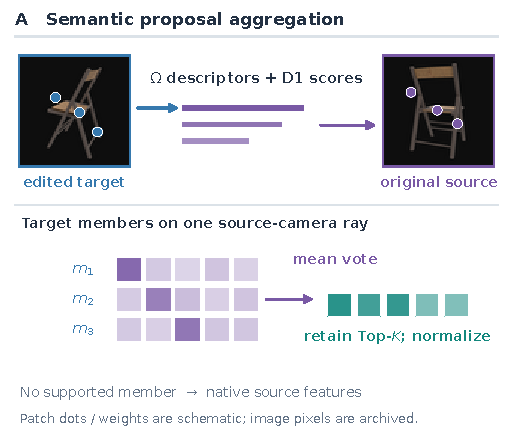
\includegraphics[width=\columnwidth]{figures/paper-matching-v2.pdf}
    \caption{\textbf{Ray-level semantic proposal aggregation.} Target patch
    members associated with one source-camera ray vote over decoder-scored
    source candidates.  We retain and normalize the aggregated Top-$K$
    posterior; an unsupported ray keeps its native source feature.}
    \label{fig:matching-aggregation}
\end{figure}
\YW{
In projection-based conditioning, a source image patch
provides the same feature to multiple 3D queries along
its camera ray.
%
However, these queries may project onto different target
patches, making their cross-geometry correspondences
ambiguous.
%
Therefore, independently matching each query yield
inconsistent source evidence, while selecting a single
best match risks missing valid correspondences.
%
To address this, we aggregate complementary matching
proposals from target patches associated with the same
source-camera ray.
%
Specifically, for each source view $j\in\mathcal{S}$,
we group voxels projecting onto the same source patch
$p$ into a ray group $r=(j,p)$.
%
We denote the distinct target patches observed through
these voxels by $\mathcal{M}_r$.
%
For each target patch $m\in\mathcal{M}_r$, the matching
decoder produces scores $s_{mk}$ over its source
candidates $\mathcal{C}_m$, which are normalized as
%
\begin{equation}
    p_m(k) =
    \frac{\exp(s_{mk}/\tau)}
    {\sum_{\ell \in \mathcal{C}_m}\exp(s_{m\ell}/\tau)},
    \label{eq:matching_probability}
\end{equation}
%
where $\tau$ is the softmax temperature and
$p_m(k)=0$ for candidates outside $\mathcal{C}_m$.
%
We aggregate these matching distributions and retain
the top-$K$ candidates:
%
\begin{equation}
    \bar{p}_r(k) =
    \frac{1}{|\mathcal{M}_r|}
    \sum_{m \in \mathcal{M}_r} p_m(k),
    \qquad
    \mathcal{K}_r = \operatorname{TopK}(\bar{p}_r).
    \label{eq:ray_matching}
\end{equation}
%
The retained scores are renormalized as
$p_r(k)=\bar{p}_r(k)/
\sum_{\ell\in\mathcal{K}_r}\bar{p}_r(\ell)$.
%
The aggregated source evidence is then computed as
%
\begin{equation}
    \mathbf{E}_r =
    \sum_{k \in \mathcal{K}_r}
    p_r(k)\mathbf{v}_k,
    \label{eq:matching_aggregation}
\end{equation}
%
where $\mathbf{v}_k$ denotes the native DINOv3 feature
used to condition the pretrained 3D generator, rather
than the VGGT-$\Omega$ descriptors used by the
separately trained matching decoder.
%
By combining matching probabilities from multiple target
patches, we aggregate relevant source features rather than
relying on a single correspondence.
%
The aggregated feature is shared across 3D queries
projecting onto the same source patch and subsequently
adapted to the target geometry through target-aware
feature retargeting.
}









































\paragraph{Target-Aware Feature Retargeting.}
%
\begin{figure}[t]
    \centering
    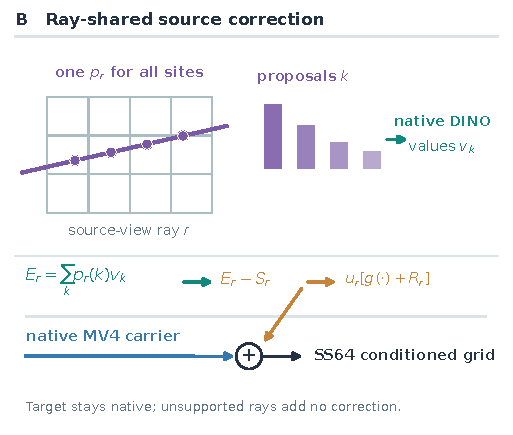
\includegraphics[width=\columnwidth]{figures/paper-retargeting-v2.pdf}
    \caption{\textbf{Ray-shared source correction.} The shared posterior
    weights native DINOv3 values to form $\mathbf{E}_r$.  A gated residual
    derived from $\mathbf{E}_r-\mathbf{S}_r$ adapts the existing source
    carrier; target conditioning remains native and unsupported rays receive
    no correction.}
    \label{fig:ray-retargeting}
\end{figure}
\YW{
Although matching-aware aggregation retrieves relevant
source appearance evidence, directly replacing the original
source features may disrupt the pretrained conditioning.
%
We therefore adapt the existing source features toward
the retrieved evidence, conditioned on the target geometry.
%
For each ray $r$, let $\mathbf{S}_r$ denote the original
source feature and $\mathbf{T}_r$ the target-view context
pooled over the corresponding 3D queries.
%
We compute the retargeted source feature as
%
\begin{equation}
    \begin{aligned}
        \mathbf{R}_r &=
        \mathcal{R}_{\phi}
        \left([\mathbf{E}_r-\mathbf{S}_r,\mathbf{T}_r]\right),\\
        \widetilde{\mathbf{S}}_r &=
        \mathbf{S}_r+
        u_r\left[
            g(\mathbf{E}_r-\mathbf{S}_r)+\mathbf{R}_r
        \right],
    \end{aligned}
    \label{eq:feature_retargeting}
\end{equation}
%
where $\mathcal{R}_{\phi}$ is a learnable retargeting
network, $u_r$ controls the use of matched evidence,
and $g$ is a bounded, signed gate.
%
The feature difference $\mathbf{E}_r-\mathbf{S}_r$
guides the source adaptation, while $\mathbf{T}_r$
provides target-specific context.
%
Rather than introducing an additional conditioning stream,
we update the existing source evidence through
a residual formulation:
%
\begin{equation}
    \mathbf{C} =
    \mathbf{C}_{\mathrm{MV}}+
    \frac{1}{V}\sum_{j\in\mathcal{S}}
    \mathcal{P}_j(
        \widetilde{\mathbf{S}}_j-\mathbf{S}_j
    ),
    \label{eq:retargeted_conditioning}
\end{equation}
%
where $\mathcal{P}_j$ projects source-view features
into the shared 3D space.
%
This formulation preserves the pretrained conditioning
at initialization while allowing source features to
be selectively adapted to the target geometry.
%
Rays without valid matching evidence retain their
original source features.
%
% Finally, we adopt stage-specific retargeting: matching-weighted Top-$K$ aggregation for geometry generation and a separately trained Top-1 retargeter for appearance synthesis, while keeping the intermediate shape stages frozen.
}
